\section{Current Status of the Framework}
By combining the presented technology stacks, the framework provides deep insights into the complete cluster stack.

\subsection{Domain Modeling}
By using a schema-less graph database approach, each domain can be modeled independently. Common entities are connected at any time after
they are modeled.

\subsubsection{Resource Scheduler}
A resource scheduler, e.g. \gls{slurm}, provides information about resource allocations: Which jobs was started where, by whom,  at what time? How long did it last? What was the outcome? and alike.
The following entities are modeled as nodes within the graph.
\begin{itemize}
    \item \textbf{host} compute node within the cluster, identified by the host-name.
    \item \textbf{partition} A logical group of nodes which represent the target of a job submission.
    \item \textbf{job} A demand for resources submitted by a user. Including metadata (user, submission/start/end time, job script, etc) and information about the state of the job. If resources are allocated, the job metadata is updated accordingly.
\end{itemize}
Relationships are added to connect certain nodes. \lstinline{PART_OF} declares host memberships to partitions. \lstinline{JOBCLIENT} connects a host to a certain running job.

\subsubsection{InfiniBand Interconnect}
An InfiniBand representation comprises of a set of physical and logical representations.
\begin{figure}[!ht]
    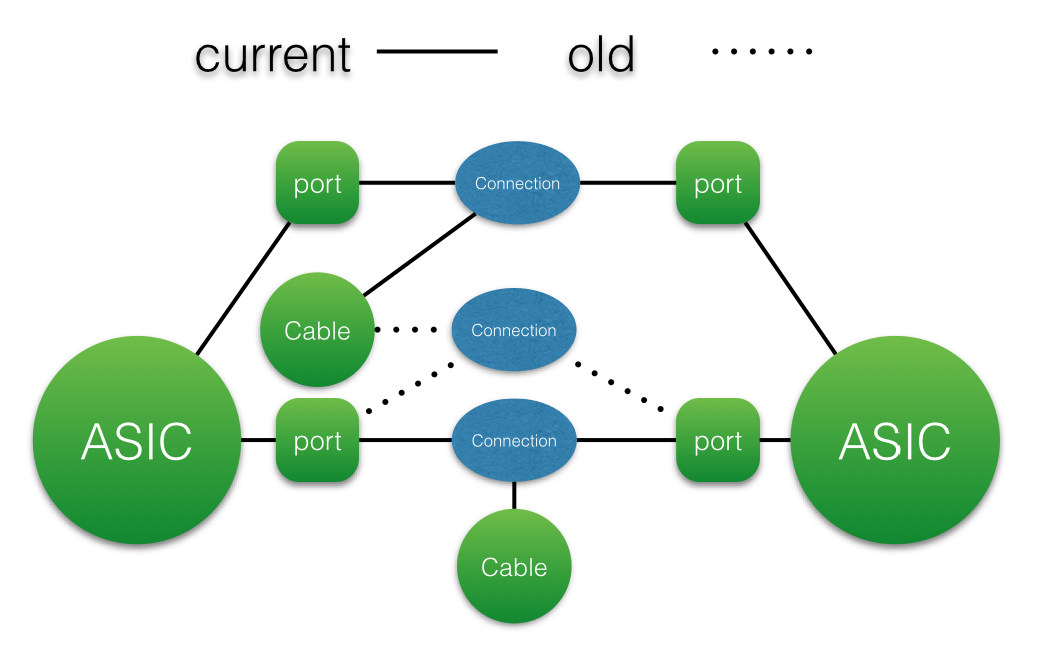
\includegraphics[width=.4\textwidth]{images/png/infiniband_graph.png}
    \caption{\label{fig:ib_graph}Modeling of an InfiniBand network.}
\end{figure}

\begin{itemize}
    \item \textbf{HCA} Network adapter plugged into a host
    \item \textbf{SW} InfiniBand switch
    \item \textbf{PORT} Each \lstinline{HCA} and \lstinline{SW} are composed of a set of ports which provide connectivity.
    \item \textbf{CABLE} Physical connection between different ports.
    \item \textbf{CONNECTION} Logical entity which connects two \lstinline{PORTS} and a \lstinline{CABLE} for a given period in time.
\end{itemize}

Relationships combine two \lstinline{PORTS} and a \lstinline{CABLE} alongside with meta-information about the time when it was created, if the connection is still valid and a like.
Furthermore the routing information is added by providing a \lstinline{ROUTE_TO} relationship between a port and a host.

\subsection{Holistic Inventory}
The presented two models alone provide combined insight into the cluster.
By connecting the HCA (within the InfiniBand model) to a host (within the \gls{slurm} model) the inventory
allows inter-layer queries.

\subsubsection{Job Placements}
By showing the layout of a job within the \gls{ib} topology, an imbalanced job is easily detectable. \autoref{fig:hop_mis} shows an example in which the hop-count within a job differs.
\begin{figure}[!ht]
    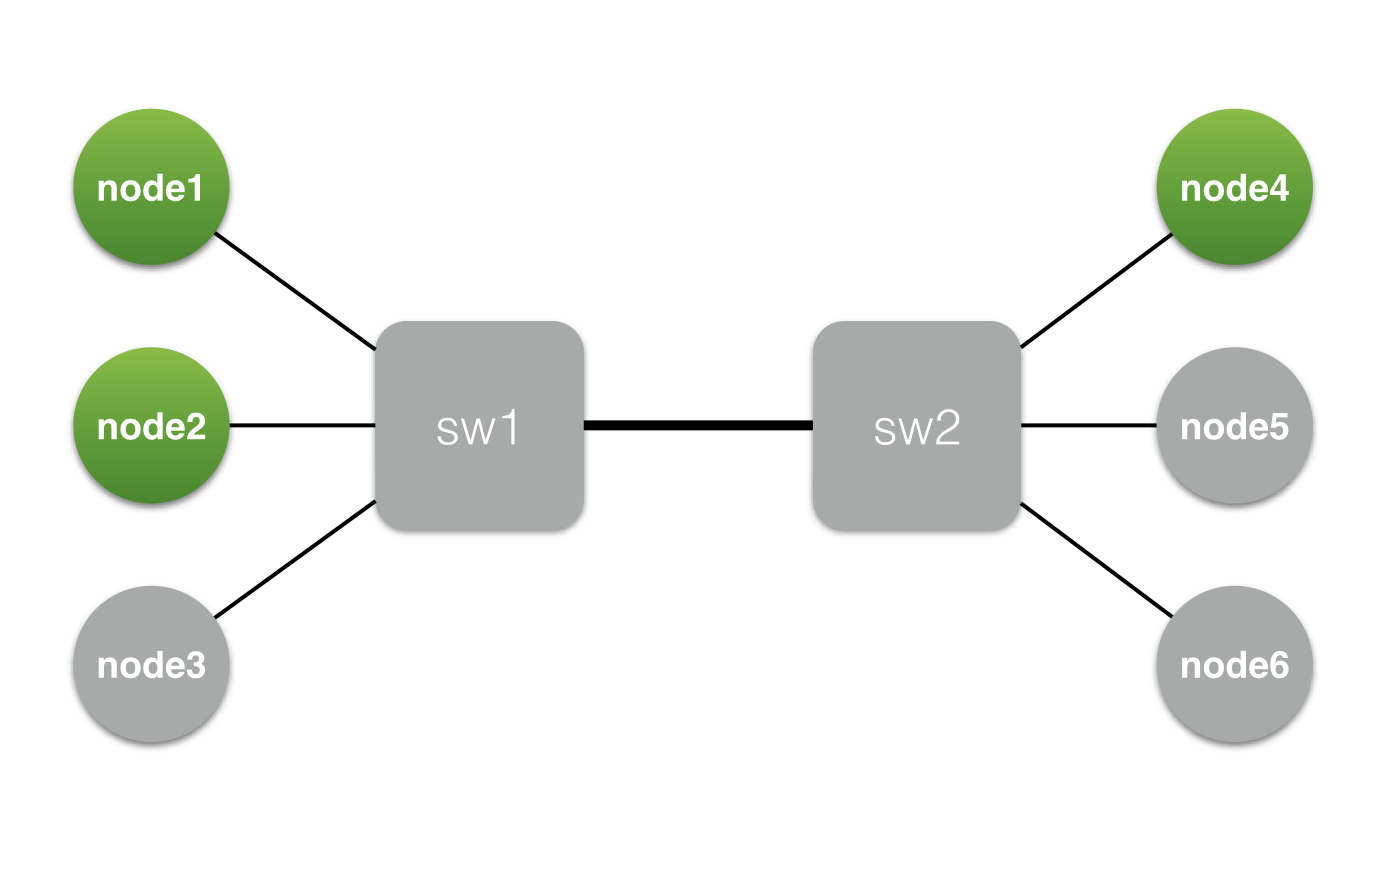
\includegraphics[width=.4\textwidth]{images/png/hop_missmatch.png}
    \caption{\label{fig:hop_mis}A job runs on three nodes (green). By using \lstinline{node3} instead of \lstinline{node4} the job could run evenly distributed on \lstinline{sw1}}
\end{figure}
A slightly more complex case would include different port-characteristics like speed or width.
By caching information of the metrics system within the graph database an even more sophisticated query
might include error or performance counters.

\subsubsection{InfiniBand Debugging}
A common debug case within the InfiniBand network is to figure out if errors associated with a connection are caused by one of the ports or the cable itself.
The typical approach to fix this error is to carefully unplug one connector of a given cable, connect it to a different switch-port and check the error counters of the just established connection.
If the error sticks with the cable the opposite side of the cable has to be changed as well, to truly pin down the problem.

This process is extremely error prone; an inventory to deal with an InfiniBand fabric barely exists. Therefore each step is manual labor with the risk of miscommunication between the on-site engineer changing the
cables and the engineer matching the changes to performance counter changes.

By using an holistic inventory (as indicated in \autoref{fig:ib_graph}) the changes are tracked automatically and since they include the timestamps the correlation with the metrics systems is trivial.

\subsection{Open Log and Metric Framework}
Determining inter-layer error triggers is an extremely hard task. If e.g. a specific job triggers an error within the interconnects one has to keep track of the job placement, the routes within the interconnect and
the time to correlate metrics with this events.

\autoref{fig:ib_perf} shows the performance metrics and the topology of the InifiniBand network,
as a first overview. Hosts which have vanished from the network are going to be marked, so that such errors are easy to spot.

\begin{figure}[!ht]
    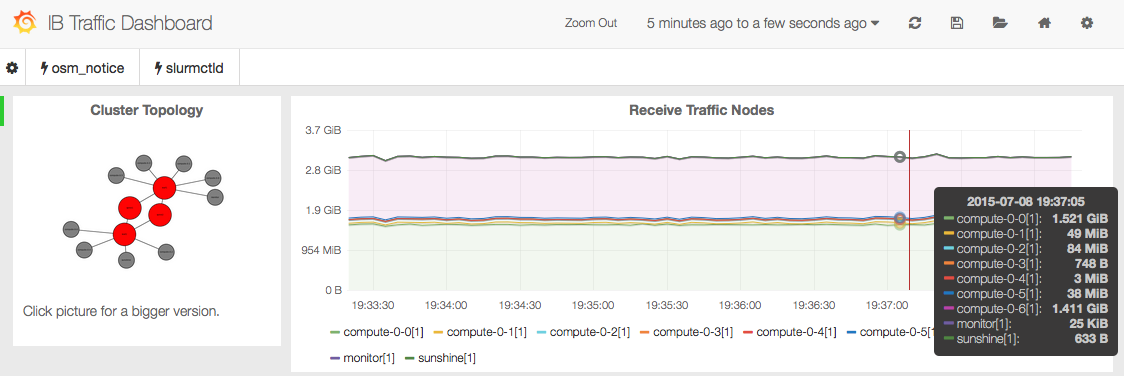
\includegraphics[width=.4\textwidth]{images/png/ib_perf_s.png}
    \caption{\label{fig:ib_perf}Dashboard to visualize the topology (left) and the live traffic metrics within the InfiniBand fabric.}
\end{figure}

\begin{figure}[!ht]
    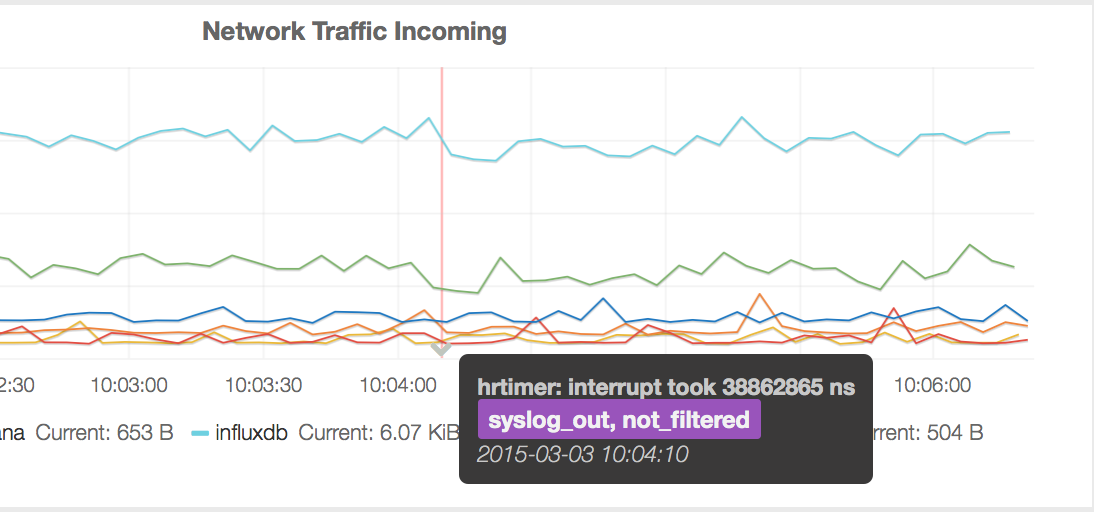
\includegraphics[width=.4\textwidth]{images/png/combined_perf.png}
    \caption{\label{fig:cor_net}Performance metrics annotated with syslog events to correlate events and metrics.}
\end{figure}
Overlaying events and metrics allows to correlate both data sources. \autoref{fig:cor_net} shows an example of an event annotated to network metrics. The slight decrease in the upper most metric might indicate causality, which is hard to spot without the overlay.